\section{Résultats du run 1 (Kaggle, GPU)}\label{sec:resultats}

Les chiffres de cette section viennent des fichiers \code{lab\_results.zip} du run 1 (6 octobre 2026). Le split est fixé : fit 104\,520, valid 24\,120, stress 16\,080, audit 16\,080 (jamais ouvert).

\subsection{Screening univarié}
\begin{table}[H]\centering\small
\begin{tabular}{lccc}
\toprule
Feature & $\eta^2$ (fit) & KS train/test & shift (sd)\\
\midrule
\code{levels:log\_depth\_q90} & 0,630 & 0,135 & $-0{,}28$\\
\code{levels:log\_depth\_q50} & 0,618 & 0,170 & $-0{,}37$\\
\code{ticks:spread\_5p} & 0,563 & \new{0,024} & $-0{,}04$\\
\code{levels:log\_depth\_q10} & 0,510 & 0,174 & $-0{,}33$\\
\code{ticks:spread\_1} & 0,504 & \new{0,018} & $+0{,}03$\\
\code{ticks:log\_spread\_t\_mean} & 0,430 & \new{0,026} & $-0{,}06$\\
\code{levels:log\_absflux\_mean} & 0,415 & 0,172 & $-0{,}37$\\
\code{position:log\_dist\_mean} & 0,363 & 0,122 & $+0{,}31$\\
\code{lots:flux\_odd} & 0,361 & 0,191 & $+0{,}45$\\
\code{lots:flux\_round} & 0,353 & 0,183 & $-0{,}42$\\
\bottomrule
\end{tabular}
\caption{Les dix colonnes les plus séparatrices. En vert : les colonnes de tick, à la fois séparatrices et stables.}
\end{table}

\begin{figure}[H]\centering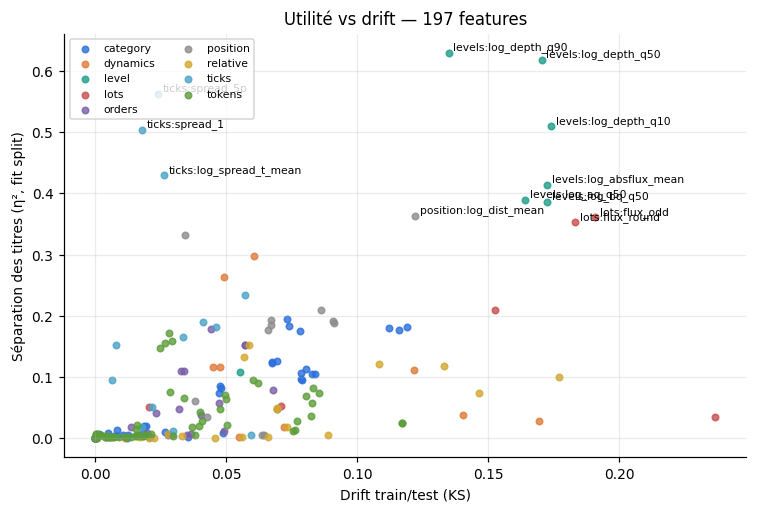
\includegraphics[width=.8\linewidth]{figures/screen_map.png}
\caption{Carte utilité/dérive des 197 colonnes.}\end{figure}

\paragraph{Trois enseignements.}
\begin{enumerate}
\item \textbf{Les ticks sont une signature stable.} $\eta^2\approx0{,}5$ avec $\mathrm{KS}\approx0{,}02$ : c'est exactement ce que la section~\ref{sec:unites} prédisait de la forme discrète du spread.
\item \textbf{La profondeur est séparatrice \emph{et} décalée.} Le test est moins profond de $0{,}3$ à $0{,}4$ écart-type.
\item \textbf{Les lots dérivent.} Le test contient davantage d'odd lots ($+0{,}45$ sd) et moins de lots ronds ($-0{,}42$ sd). Avec la baisse de profondeur, c'est cohérent avec l'hypothèse de prix plus élevés (section~\ref{sec:aug}).
\end{enumerate}

\subsection{AUC adversariale}
\begin{table}[H]\centering\small
\begin{tabular}{lcc|lcc}
\toprule
Bloc & $d$ & AUC & Bloc & $d$ & AUC\\
\midrule
\code{base\_relative} & 18 & 0,733 & \code{book\_dyn} & 10 & 0,669\\
\code{levels} & 7 & 0,709 & \code{cat\_cross} & 30 & 0,668\\
\code{lots} & 9 & 0,699 & \code{cat\_freq} & 12 & 0,668\\
\code{position} & 15 & 0,670 & \code{transitions} & 36 & 0,653\\
\code{tokens\_bow} & 24 & 0,618 & \code{orders} & 22 & 0,596\\
\code{ticks} & 14 & \new{0,568} & \textbf{tous} & 197 & \textbf{0,863}\\
\bottomrule
\end{tabular}
\caption{Séparabilité train/test, bloc par bloc. Le total (0,863) est cohérent avec l'ancienne AUC CatBoost (0,903). Aucun bloc seul n'explique le décalage : il est diffus.}
\end{table}
Fait notable : la base relative du pipeline précédent est \emph{la plus} décalée (0,733). Être invariant à l'échelle ne garantit pas d'être stable entre périodes.

\subsection{Ajout réentraîné}
Base \code{base\_relative}+\code{cat\_freq} : valid 0,313, stress 0,245 (XGBoost, 50\,\% du fit).
\begin{table}[H]\centering\small
\begin{tabular}{lrrrr}
\toprule
+ bloc & $\Delta$ valid & IC 95\,\% & $\Delta$ stress & retenu ?\\
\midrule
\code{position} & +5,9 & [+5,3 ; +6,4] & +3,8 & oui\\
\code{levels} & +5,4 & [+4,9 ; +5,9] & \old{$-13{,}3$} & \old{non}\\
\code{lots} & +5,2 & [+4,7 ; +5,8] & +4,3 & oui\\
\code{ticks} & +5,0 & [+4,5 ; +5,5] & \new{+5,3} & oui\\
\code{tokens\_bow} & +3,6 & [+3,1 ; +4,2] & +2,1 & oui\\
\code{book\_dyn} & +3,5 & [+3,0 ; +4,0] & $-0{,}1$ & oui\\
\code{transitions} & +2,0 & [+1,5 ; +2,5] & +1,7 & oui\\
\code{orders} & +1,5 & [+1,0 ; +1,9] & +0,8 & oui\\
\code{cat\_cross} & +0,6 & [+0,2 ; +1,1] & +0,4 & oui\\
\bottomrule
\end{tabular}
\caption{En points d'accuracy. \code{levels} est le seul bloc écarté par la règle : il fait gagner 5,4 points en validation et en perdre 13,3 en stress. C'est un piège de régime.}
\end{table}

\begin{figure}[H]\centering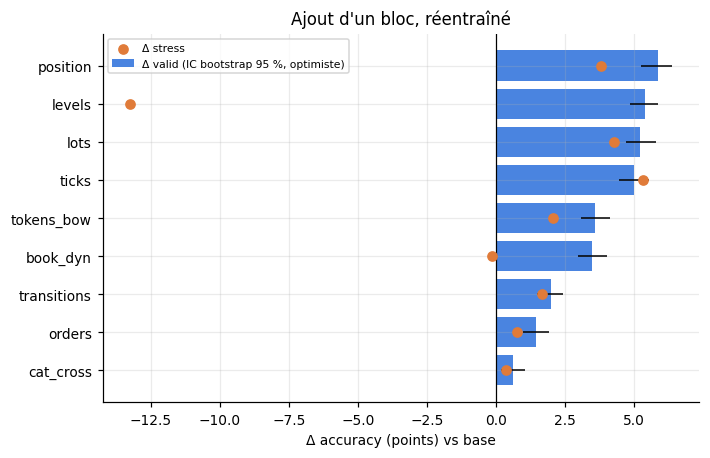
\includegraphics[width=.75\linewidth]{figures/screen_forward.png}\caption{Ajout réentraîné, valid et stress.}\end{figure}

\subsection{Retrait réentraîné}
Sur les 10 blocs retenus (190 colonnes) : valid 0,465, stress 0,364.
\begin{table}[H]\centering\small
\begin{tabular}{lrr|lrr}
\toprule
$-$ bloc & $\Delta$ valid & $\Delta$ stress & $-$ bloc & $\Delta$ valid & $\Delta$ stress\\
\midrule
\code{lots} & $-4{,}1$ & $-3{,}1$ & \code{book\_dyn} & $-0{,}7$ & $-0{,}1$\\
\code{base\_relative} & $-2{,}3$ & $-0{,}05$ & \code{transitions} & $-0{,}7$ & $-0{,}1$\\
\code{ticks} & $-1{,}4$ & $-1{,}6$ & \code{tokens\_bow} & $-0{,}4$ & $0{,}0$\\
\code{orders} & $-1{,}2$ & $-0{,}6$ & \code{cat\_freq} & $-0{,}2$ & $-0{,}3$\\
\code{position} & $-0{,}9$ & $-0{,}5$ & \code{cat\_cross} & $+0{,}1$ & $-0{,}2$\\
\bottomrule
\end{tabular}
\caption{En points. \code{cat\_cross}, \code{cat\_freq} et \code{tokens\_bow} sont redondants une fois les autres blocs présents.}
\end{table}

\subsection{Modèles}
\begin{table}[H]\centering\small
\begin{tabular}{lrrrrrr}
\toprule
Run & Param. & Ép. & Min & Valid & Stress & Stress éq.\\
\midrule
\code{tab\_lgbm} & — & 266 it. & 3,7 & 0,480 & 0,372 & —\\
\code{tab\_xgb} & — & 711 it. & 1,4 & 0,494 & 0,384 & —\\
\code{tab\_mlp} & — & 14 & 0,1 & 0,511 & 0,390 & —\\
\code{control\_gru\_s0} & 110\,105 & 39 & 3,2 & 0,787 & 0,662 & —\\
\code{signature\_relative\_only\_s0} & 340\,289 & 38 & 10,4 & 0,766 & 0,669 & —\\
\code{signature\_no\_bias\_s0} & 342\,905 & 40 & 8,6 & 0,824 & 0,716 & —\\
\code{signature\_s0} & 342\,913 & 38 & 10,4 & 0,825 & 0,712 & —\\
\code{signature\_s1} & 342\,913 & 37 & 10,4 & 0,827 & 0,730 & —\\
\code{signature\_robust\_s0} & 342\,913 & 39 & 10,5 & 0,830 & 0,689 & —\\
\code{signature\_robust\_s1} & 342\,913 & 35 & 10,5 & 0,836 & 0,719 & —\\
\midrule
\textbf{blend des 4 finalistes} & & & & 0,852 & 0,741 & 0,806\\
\bottomrule
\end{tabular}
\caption{Run 1. La colonne « stress éq. » (après Sinkhorn) n'a été calculée que pour le blend : elle devient le critère de sélection au round 2.}
\end{table}

\paragraph{Lecture prudente.}
\begin{itemize}
\item \textbf{Séquence contre tabulaire} : 0,79--0,84 contre 0,48--0,51 en validation. Lire les événements apporte beaucoup plus que des statistiques de fenêtre. Mais la validation aléatoire profite aussi davantage aux modèles séquentiels, qui reconnaissent mieux le jour (section~\ref{sec:dependance}).
\item \textbf{\code{signature} contre \code{control\_gru}} : +3,8 points en valid, +5,0 en stress. Mais le rapport de paramètres est de $3{,}1$. Design et capacité sont confondus : c'est l'objet de \code{gru\_wide} au round 2.
\item \textbf{Biais « même ordre »} : 0,8251 avec, 0,8238 sans. L'écart est plus petit que celui entre graines (0,8251 et 0,8266). Pas d'effet mesurable : le retirer simplifie le modèle.
\item \textbf{Robustesse} (venue dropout, jitter, dropout de blocs) : +0,7 point en valid en moyenne, $-1{,}7$ en stress. Pas de gain de transfert.
\item \textbf{Niveaux} : les retirer coûte 5,9 points en valid et 4,3 en stress (une seule graine).
\item \textbf{Maturité} : la meilleure époque tombe entre 35 et 40, mais c'est la fin du cosinus qui aplatit la courbe. L'écart en mode \code{eval} est de 0,91 (train) contre 0,82 (valid).
\end{itemize}

\begin{figure}[H]\centering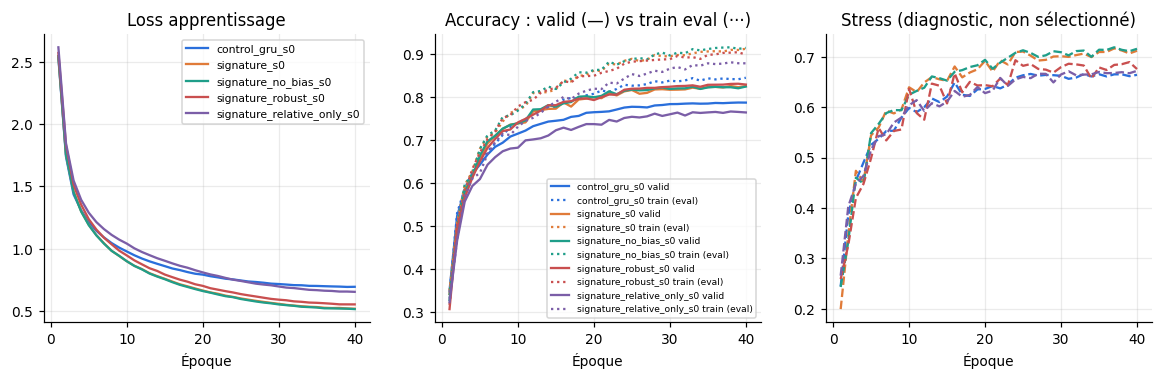
\includegraphics[width=\linewidth]{figures/histories.png}\caption{Courbes d'apprentissage (seed 0). Le stress est tracé mais ne sélectionne rien.}\end{figure}
\begin{figure}[H]\centering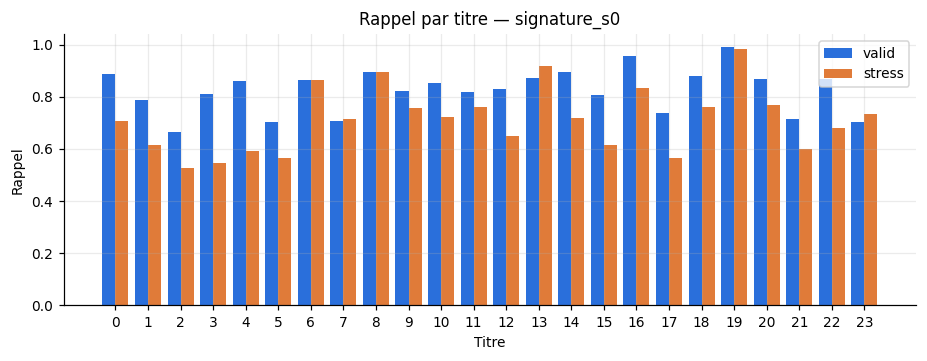
\includegraphics[width=.9\linewidth]{figures/recall_signature_s0.png}\caption{Rappel par titre, \code{signature\_s0}.}\end{figure}

\subsection{Du stress au leaderboard}
\begin{figure}[H]\centering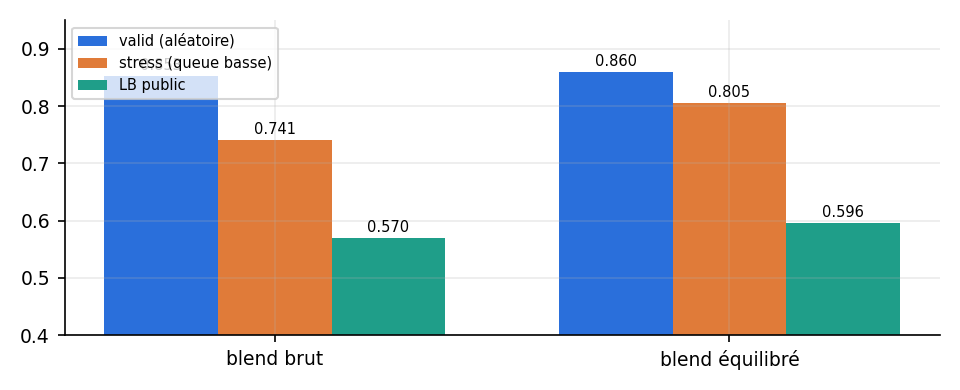
\includegraphics[width=.75\linewidth]{figures/valid_stress_lb.png}
\caption{Les trois mesures pour les deux soumissions. Le classement relatif (brut < équilibré) est le même partout. L'écart absolu, lui, ne l'est pas.}\end{figure}
L'écart validation → LB est de 28 points. L'écart stress → LB est de 17 points (brut) et de 21 points (équilibré). Aucune partition interne n'estime donc le score public. En revanche, le stress a correctement \emph{ordonné} les deux variantes. C'est pourquoi le round 2 classe les configurations sur le stress équilibré, et ancre les indicateurs sans labels sur les deux scores connus.
